\documentclass[11pt,a4paper,oneside]{book}
%
%--------------------   start of the 'preamble'
%
\usepackage{graphicx,amssymb,amstext,amsmath,float,color,array,ctable,booktabs,wrapfig,caption}
%
\usepackage[table]{xcolor}
\usepackage{graphics}
\usepackage{hyperref}
\usepackage{pgf}
\usepackage{natbib}
\usepackage{verbatim}
\usepackage{titlesec}
\titleformat{\chapter}[hang] 
{\normalfont\huge\bfseries}{\ \thechapter}{1em}{} 
\usepackage{tikz}
\usetikzlibrary{shapes}
\usetikzlibrary{calc,backgrounds}
\usetikzlibrary{automata}
\usetikzlibrary{arrows,positioning,calc,matrix} 
\usetikzlibrary{decorations.pathreplacing,shapes.multipart}

\tikzstyle{Dstate}=[shape=circle,draw=black!50,fill=black!10]
\tikzstyle{Istate}=[shape=diamond,draw=black!50,fill=black!10]
\tikzstyle{Mstate}=[shape=rectangle,draw=black!50,fill=black!10]

\tikzstyle{empty}=[shape=circle]

\tikzstyle{lightedge}=[->,dotted,thick]
\tikzstyle{mainstate}=[state,thick]
\tikzstyle{mainedge}=[->,thick]

\definecolor{black}{RGB}{0,0,0}
\definecolor{darkgrey}{RGB}{64,64,64}
\definecolor{grey}{RGB}{127,127,127}
\definecolor{lightgrey}{RGB}{230,230,230}

% scheme 1 
\definecolor{winered}{RGB}{158,16,0}
\definecolor{lightred}{RGB}{199,53,42}
\definecolor{brown}{RGB}{158,95,0}
\definecolor{orange}{RGB}{235,141,0}

%scheme2

\definecolor{darkblue}{RGB}{19,48,182}

\definecolor{blue}{RGB}{36,89,158}
\definecolor{browngreen}{RGB}{82,75,19}
\definecolor{lightbrown}{RGB}{158,126,36}

%scheme3

\definecolor{green}{RGB}{52,132,23}


\definecolor{lightgreen}{RGB}{82,209,36}
\definecolor{lightbrowngreen}{RGB}{125,133,23}
\definecolor{yellowgreen}{RGB}{198,209,36}

%scheme4


\definecolor{paper}{RGB}{240,238,183}
\definecolor{organicgrey}{RGB}{163,162,124}


\definecolor{metal}{RGB}{75,81,82}


\setlength{\parindent}{0cm}
\pagestyle{empty}

\makeindex
\usepackage{anysize}

%\marginsize{left}{right}{top}{bottom}:
\marginsize{2cm}{2cm}{2cm}{2cm}

\newcommand{\aln}[2]{\shortstack{ #1\\  #2}}

\begin{document}
\frontmatter
%-----------------------------------------------------------
\newlength{\centeroffset}
%\setlength{\centeroffset}{-0.5\oddsidemargin}
%\addtolength{\centeroffset}{0.5\evensidemargin}
%\addtolength{\textwidth}{-\centeroffset}
\thispagestyle{empty}
\vspace*{\stretch{1}}
\noindent\hspace*{\centeroffset}\makebox[0pt][l]{\begin{minipage}{\textwidth}
\flushright
{\Huge\bfseries 

The TagDust2 Manual

}


\end{minipage}}

\vspace{\stretch{1}}
\noindent\hspace*{\centeroffset}\makebox[0pt][l]{\begin{minipage}{\textwidth}
\flushright


\vspace{\stretch{1}}
{\bfseries 
by Timo Lassmann\\[1.5ex]} 
\noindent\rule[-1ex]{\textwidth}{1pt}\\[2.5ex]
 \today

\end{minipage}}

%\addtolength{\textwidth}{\centeroffset}
%\vspace{\stretch{2}}


\pagebreak
\begin{small} 

Copyright \copyright 2013 Timo Lassmann (timolassmann@gmail.com)
 
 This document is free;  you can redistribute it and/or modify
 it under the terms of the GNU General Public License as published by
 the Free Software Foundation, either version 3 of the License, or
 (at your option) any later version.
 
 This document is distributed in the hope that it will be useful,
 but WITHOUT ANY WARRANTY; without even the implied warranty of
 MERCHANTABILITY or FITNESS FOR A PARTICULAR PURPOSE.  See the
 GNU General Public License for more details.
 
 You should have received a copy of the GNU General Public License
 along with TagDust.  
 
 If not, see (http://www.gnu.org/licenses/).



\end{small}

%-----------------------------------------------------------
\tableofcontents
%-----------------------------------------------------------
\mainmatter
%\setcounter{chapter}{-1}

%\setcounter{chapter}{1}
%\setcounter{section}{0}
\chapter{Introduction}

 %\addcontentsline{toc}{chapter}{Introduction}

Raw sequences produced by next generation sequencing (NGS) machines may contain adapter, linker, barcode and fingerprint sequences. TagDust2 is a program to extract and correctly label the sequences to be mapped in downstream pipelines.

TagDust allows users to specify the expected architecture of a read and converts it into a hidden Markov model. The latter can assign sequences to a particular barcode (or index) even in the presence of sequencing errors. Sequences not matching the architecture (primer dimers, contaminants etc.) are automatically discarded (see Figure \ref{figure1}).


%\begin{wrapfigure}{l}{1\textwidth}

\begin{figure}[h]


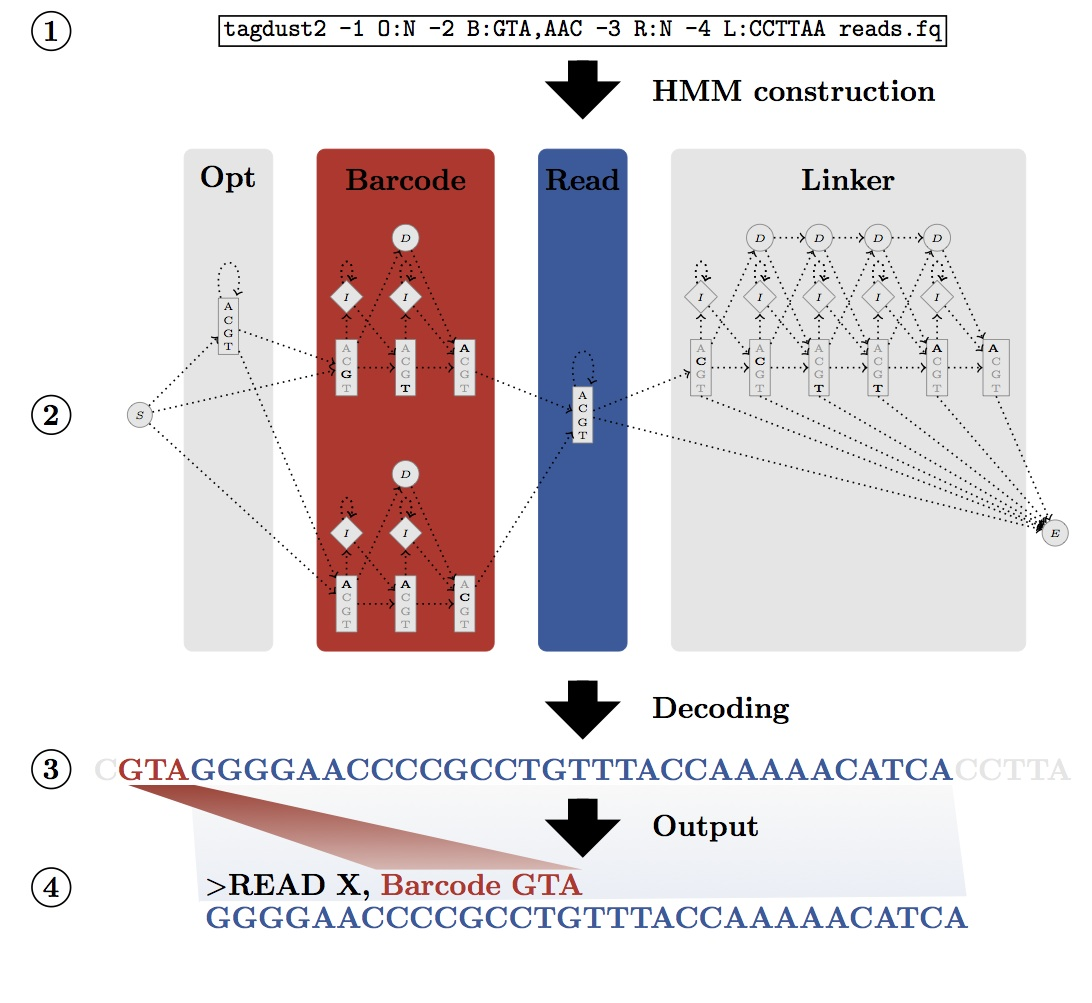
\includegraphics[scale = 0.9]{figures/figure1.pdf}

\caption{A HMM specifies the expected architecture of the raw sequence. After decoding sequences are segmented into the components of the architecture. Based on the segmentation, a barcode is assigned to each read and remaining sequences are trimmed.}
\label{figure1}
\end{figure}


%\end{wrapfigure}

\newpage

\chapter{Installation}
%\addcontentsline{toc}{chapter}{Installation}


%\section*{Quick installation instructions}
%\addcontentsline{toc}{section}{Quick installation instructions}
Unpack the tarball:

\begin{verbatim}
bash-3.1$ tar -zxvf tagdust-2.04.tar.gz 
\end{verbatim}

\begin{verbatim}
bash-3.1$ cd tagdust
\end{verbatim}


\begin{verbatim}
bash-3.1$ ./configure
\end{verbatim}
\begin{verbatim}
bash-3.1$ make
\end{verbatim}
At this point the TagDust executable appears in the TagDust directory. You can copy it to any directory in your path. To install it system wide type:  
\begin{verbatim}
bash-3.1$ make install
\end{verbatim}
%\let\clearpage\relax
\chapter{Usage}

\section{Command Line}
TagDust requires an input file containing sequences and a user specified HMM architecture used to extract the reads. For the architecture all that TagDust needs to know is the sequence of pre-defined building blocks. Options '{\tt -1,-2, ...}' are used to specify the first, second, etc. building block.

\begin{verbatim}
bash-3.1$ tagdust [-options] <input file>  
\end{verbatim}

\rowcolors{1}{lightgrey}{white}

\begin{center}
\begin{tabular}{| l | l | p{12cm}|}
\hline
\rowcolor{blue} \textcolor{white}{\scshape Option}		&\textcolor{white}{\scshape Type}		&	\textcolor{white}{\scshape Description}\\ \hline
-Q & FLT & read quality threshold [20].\\
-start & INT & start of search area [0].\\
-end & INT & end of  search area [length of sequence].\\
-format & STR & format of input sequence file.\\
-minlen & INT & minimal accepted read length [16].\\
-ref     &  STR &    reference fasta file to be compared against[].\\
-fe &       INT &    number of errors allowed when comparing to reference[2].\\
-dust &	INT &	remove low complexity sequences[].\\
-e & FLT & expected sequencer error rate [0.05].\\ 
-o & STR & output file name.\\
-t & INT & number of threads [8].\\
-1 & STR & type of the first HMM building block. \\
-2 & STR & type of the second HMM building block.\\
-\dots & STR & type of the \dots HMM building block.\\
\hline
\end{tabular}
\end{center}
\section{Notes}
\subsection{Threshold}
The {\tt -Q} option sets the minimum acceptable read quality analogous to the mapping quality Q. If the reads are very short or the model very simple (e.g. 3 nucleotide barcode followed by the read) the default threshold of 20 might have to be lowered.

\subsection{Removing Known Contaminants (e.g. ribosomal RNA sequences).}
Known contaminants or unwanted reads can be filtered from the output by pointing TagDust to a reference fasta to be matched against ({\tt -ref <filename>} ). The maximum number of errors allowed for a match to reference is set with the {\tt -fe} option.
\subsection{Removing Low Complexity Sequences}
Tagdust implements a simplified version of the DUST module (R. Tatusov and D.J. Lipman, unpublished data) to filter out low complexity reads. While this is not strictly necessary for NGS reads I implemented it to remove poly-A and other "very" low complexity sequences. The algorithm is only applied to the first 64 nucleotides of the reads. The {\tt -dust} option both enables and sets the threshold for the low complexity filtering. I recommend using a relaxed threshold of 100 and leave the rest to the downstream mapping algorithm. 


\subsection{Efficiency}
As a default, TagDust attempts to match the entire sequence to the HMM (global). The options {\tt -start} and {\tt -end} restricts the matching to region specified. TagDust assumes that all residues upstream of 'start' do not belong to the read while all residues following 'end' are read residues.

In the presence of barcodes or fingerprints, TagDust will recognize the most likely code and append it to the name of the read. 

\section{Formats}
\subsection{Input file formats}

TagDust can work with fasta, fastq and SAM/BAM files. Gzipped files are also supported. The format is automatically recognized by the file suffix. If the input is streamed, the '{\tt -format}' option has to be used to specify the format.\\
 
\subsection{Output format}
The output format is always a fastq file. If barcodes or fingerprints are present, TagDust appends them to the read name: 

{\small
\begin{verbatim}
@110922_SN549_0034_BB03F7ABXX:7:1101:1137:1974#0/1 BC:AGT;FP:367
CNCTGAAACGTAGATATAGGGGAACCCCGCCTGTTTACCAAAAACATCACCTCTAGCAT
+
bBS`cceegggggiiiiiiiiiiiiiiiiiiiihhihhhiihhhiiihiiihiiiiggg
\end{verbatim}
}

Note that BC:[A,C,G,T]+ is the sequence of the barcode and FP:[0-9]+ is the fingerprint sequence converted into a unique decimal number.
\newpage

\section{HMM Building Blocks}
TagDust comes with a set of pre-defined HMM building blocks. Each includes a silent state at the beginning and end used to link blocks together. Each block is specified by a unique letter following by a colon and some information about the sequence. 


\subsection{Read}
Segment modeling the read. \\

\begin{figure}[H]
\centering
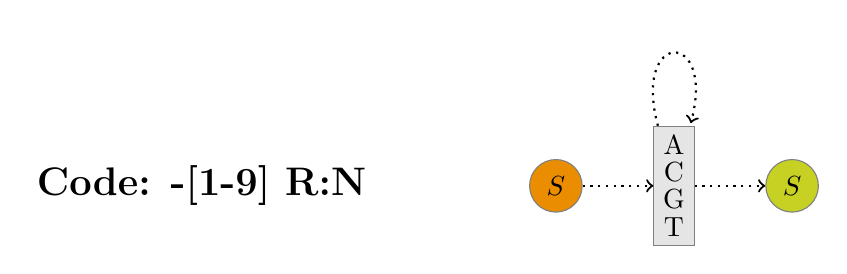
\begin{tikzpicture}
 
  \node  at (-6,0)  [font=\Large,style={align=center}] () {{\bf Code: -[1-9] R:N}};
 
\node[Dstate,fill=orange] (START) at (-1.5,0){$S$};

\node[Mstate] (O1) at (0,0){\shortstack{ A\\   C\\  G\\ T} };

\node[Dstate,fill=yellowgreen] (END) at (1.5,0){$S$};

 \path 

(START) edge [lightedge] (O1) 
(O1) edge [lightedge] (END) 

   
(O1) edge [lightedge,loop above] ();

\end{tikzpicture}
\end{figure}

\subsection{Optional}
Segment modeling an optional single or short stretch of nucleotides.  \\
Example code: O:N\\


\begin{figure}[H]
\centering
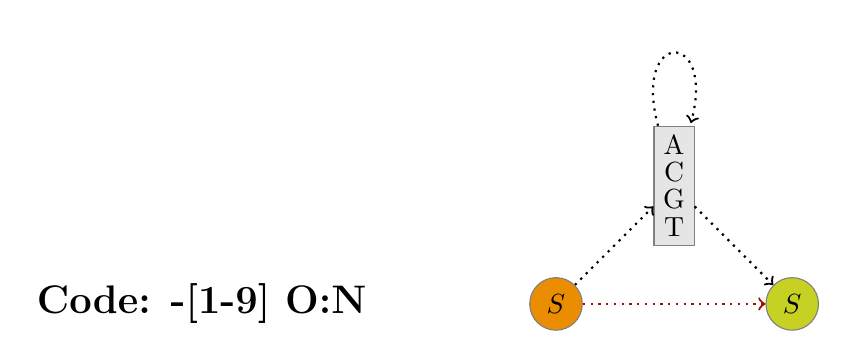
\begin{tikzpicture}
 
 \node  at (-6,0)  [font=\Large,style={align=center}] () {{\bf Code: -[1-9] O:N}};
 
\node[Dstate,fill=orange] (START) at (-1.5,0){$S$};

\node[Mstate] (O1) at (0,1.5){\shortstack{ A\\   C\\  G\\ T} };

\node[Dstate,fill=yellowgreen] (END) at (1.5,0){$S$};

 \path 

(START) edge [lightedge] (O1) 
(O1) edge [lightedge] (END) 
(START) edge [winered,lightedge] (END)
   
(O1) edge [lightedge,loop above] ();

\end{tikzpicture}
\end{figure}


\subsection{G addition}
Segment modeling the occasional addition of guanines to the reads. (89.3\% chance of a single G , 19.5 \% chance of  2 Gs..).\\
Example code: O:N\\


\begin{figure}[H]
\centering
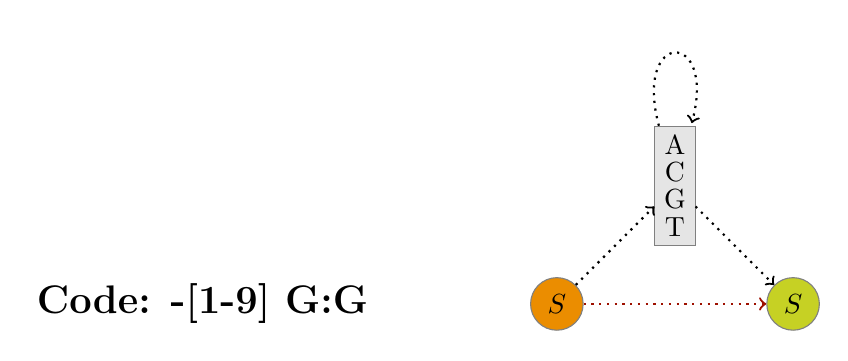
\begin{tikzpicture}
 
 \node  at (-6,0)  [font=\Large,style={align=center}] () {{\bf Code: -[1-9] G:G}};
 
\node[Dstate,fill=orange] (START) at (-1.5,0){$S$};

\node[Mstate] (O1) at (0,1.5){\shortstack{ A\\   C\\  G\\ T} };

\node[Dstate,fill=yellowgreen] (END) at (1.5,0){$S$};

 \path 

(START) edge [lightedge] (O1) 
(O1) edge [lightedge] (END) 
(START) edge [winered,lightedge] (END)
   
(O1) edge [lightedge,loop above] ();

\end{tikzpicture}
\end{figure}


\newpage 


\subsection{Barcode or Index}

Segment modeling a set of barcode sequences. For each sequence a separate HMM is created. The barcode sequences must be given as a comma separated list. A null model of the same length as the barcode is automatically added and initialized to the background nucleotide frequencies. \\



\begin{figure}[H]
\centering
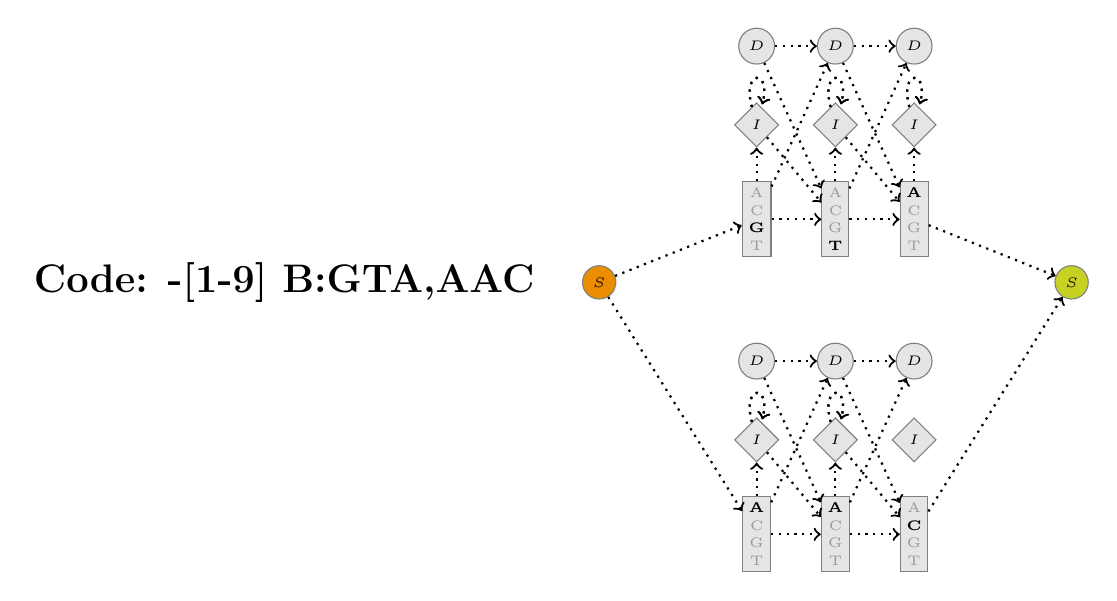
\begin{tikzpicture}
 \tiny
 
 \node  at (-7,0)  [font=\Large,style={align=center}] () {{\bf Code: -[1-9] B:GTA,AAC}};
 
 \node[Dstate,fill=orange] (START) at (-3,0){$S$};
 
\node[Dstate,fill=yellowgreen] (END) at (3,0){$S$};
 
\begin{scope}[shift={(-1,2)}];
\node[Dstate] (d1) at (0,1){$D$};
\node[Istate] (i1) at (0,0){$I$};
\node[Mstate] (m1) at (0,-1.2){\shortstack{ {\color{black!40}A}\\   {\color{black!40}C}\\  {\bf G}\\   {\color{black!40}T}} };



\node[Dstate] (d2) at (1,1){$D$};
\node[Istate] (i2) at (1,0){$I$};
\node[Mstate] (m2) at (1,-1.2){\shortstack{ {\color{black!40}A}\\   {\color{black!40}C}\\   {\color{black!40}G}\\   {\bf T}} };


\node[Dstate] (d3) at (2,1){$D$};
\node[Istate] (i3) at (2,-0){$I$};
\node[Mstate] (m3) at (2,-1.2){\shortstack{ {\bf A}\\   {\color{black!40}C}\\   {\color{black!40}G}\\   {\color{black!40}T}} };
\end{scope}


\begin{scope}[shift={(-1,-2)}];

\node[Dstate] (d4) at (0,1){$D$};
\node[Istate] (i4) at (0,0){$I$};
\node[Mstate] (m4) at (0,-1.2){\shortstack{ {\bf A}\\   {\color{black!40}C}\\   {\color{black!40}G}\\   {\color{black!40}T}} };



\node[Dstate] (d5) at (1,1){$D$};
\node[Istate] (i5) at (1,0){$I$};
\node[Mstate] (m5) at (1,-1.2){\shortstack{ {\bf A}\\   {\color{black!40}C}\\   {\color{black!40}G}\\   {\color{black!40}T}} };


\node[Dstate] (d6) at (2,1){$D$};
\node[Istate] (i6) at (2,-0){$I$};
\node[Mstate] (m6) at (2,-1.2){\shortstack{ {\color{black!40}A}\\   {\bf C}\\   {\color{black!40}G}\\   {\color{black!40}T}} };
\end{scope}

\path
(START)  edge [lightedge] (m1) 
(START)  edge [lightedge] (m4) 

(m3)  edge [lightedge] (END) 
(m6)  edge [lightedge] (END) 
(m1) edge [lightedge] (m2) 
(m1) edge [lightedge] (d2) 
(m1) edge [lightedge] (i1)
   
(i1) edge [lightedge,loop above] ()
(i1) edge  [lightedge] (m2)
(i1) edge [lightedge, loop above] ()
(d1) edge  [lightedge,->] (d2)
(d1) edge  [lightedge,->] (m2)

(m2) edge [lightedge] (m3) 
(m2) edge [lightedge] (d3) 
(m2) edge [lightedge] (i2)
   
(i2) edge [lightedge,loop above] ()
(i2) edge  [lightedge] (m3)
(i2) edge [lightedge, loop above] ()
(d2) edge  [lightedge,->] (d3)
(d2) edge  [lightedge,->] (m3)


(m3) edge [lightedge] (i3)
   
(i3) edge [lightedge,loop above] ()

(i3) edge [lightedge, loop above] ()


(m4) edge [lightedge] (m5) 
(m4) edge [lightedge] (d5) 
(m4) edge [lightedge] (i4)
   
(i4) edge [lightedge,loop above] ()
(i4) edge  [lightedge] (m5)
(i4) edge [lightedge, loop above] ()
(d4) edge  [lightedge,->] (d5)
(d4) edge  [lightedge,->] (m5)

(m5) edge [lightedge] (m6) 
(m5) edge [lightedge] (d6) 
(m5) edge [lightedge] (i5)
   
(i5) edge [lightedge,loop above] ()
(i5) edge  [lightedge] (m6)
(i5) edge [lightedge, loop above] ()
(d5) edge  [lightedge,->] (d6)
(d5) edge  [lightedge,->] (m6);



\end{tikzpicture}
\end{figure}

\subsection{Fingerprint or {\underline U}nique {\underline M}olecular {\underline I}dentifier - UMI}

Segment modeling a fingerprint (or unique molecular identifiers). Insertions and deletions are by default not allowed within a fingerprint segment.

\begin{figure}[H]
\centering
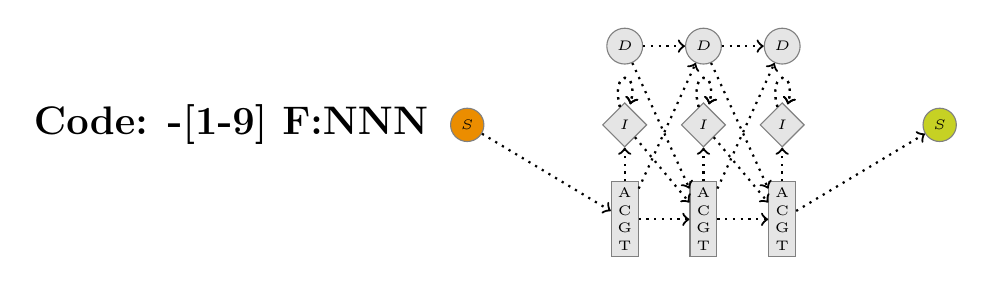
\begin{tikzpicture}
 \tiny
 
  \node  at (-6,0)  [font=\Large,style={align=center}] () {{\bf Code: -[1-9] F:NNN}};
 \node[Dstate,fill=orange] (START) at (-3,0){$S$};
 
\node[Dstate,fill=yellowgreen] (END) at (3,0){$S$};
 
\begin{scope}[shift={(-1,0)}];
\node[Dstate] (d1) at (0,1){$D$};
\node[Istate] (i1) at (0,0){$I$};
\node[Mstate] (m1) at (0,-1.2){\shortstack{ A\\   C\\  G\\ T} };



\node[Dstate] (d2) at (1,1){$D$};
\node[Istate] (i2) at (1,0){$I$};
\node[Mstate] (m2) at (1,-1.2){\shortstack{ A\\   C\\  G\\ T}};


\node[Dstate] (d3) at (2,1){$D$};
\node[Istate] (i3) at (2,-0){$I$};
\node[Mstate] (m3) at (2,-1.2){\shortstack{ A\\   C\\  G\\ T}};
\end{scope}

\path
(START)  edge [lightedge] (m1) 


(m3)  edge [lightedge] (END) 

(m1) edge [lightedge] (m2) 
(m1) edge [lightedge] (d2) 
(m1) edge [lightedge] (i1)
   
(i1) edge [lightedge,loop above] ()
(i1) edge  [lightedge] (m2)
(i1) edge [lightedge, loop above] ()
(d1) edge  [lightedge,->] (d2)
(d1) edge  [lightedge,->] (m2)

(m2) edge [lightedge] (m3) 
(m2) edge [lightedge] (d3) 
(m2) edge [lightedge] (i2)
   
(i2) edge [lightedge,loop above] ()
(i2) edge  [lightedge] (m3)
(i2) edge [lightedge, loop above] ()
(d2) edge  [lightedge,->] (d3)
(d2) edge  [lightedge,->] (m3)


(m3) edge [lightedge] (i3)
   
(i3) edge [lightedge,loop above] ()

(i3) edge [lightedge, loop above] ();




\end{tikzpicture}
\end{figure}

\subsection{Spacer}

Segment modeling a pre-defined sequence. 


\begin{figure}[H]
\centering
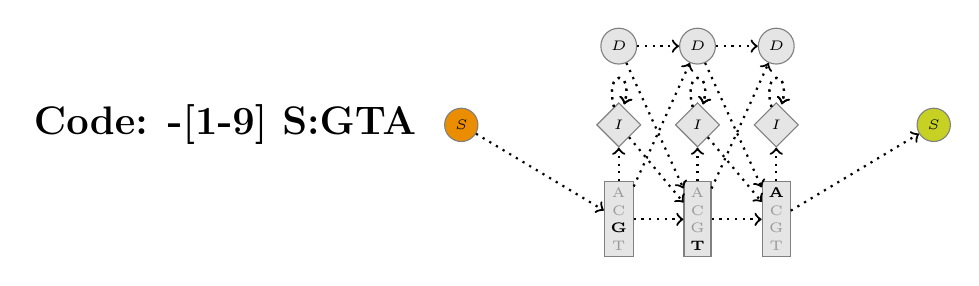
\begin{tikzpicture}
 \tiny
  \node  at (-6,0)  [font=\Large,style={align=center}] () {{\bf Code: -[1-9] S:GTA}};
 
 \node[Dstate,fill=orange] (START) at (-3,0){$S$};
 
\node[Dstate,fill=yellowgreen] (END) at (3,0){$S$};
 
\begin{scope}[shift={(-1,0)}];
\node[Dstate] (d1) at (0,1){$D$};
\node[Istate] (i1) at (0,0){$I$};
\node[Mstate] (m1) at (0,-1.2){\shortstack{ {\color{black!40}A}\\   {\color{black!40}C}\\  {\bf G}\\   {\color{black!40}T}} };



\node[Dstate] (d2) at (1,1){$D$};
\node[Istate] (i2) at (1,0){$I$};
\node[Mstate] (m2) at (1,-1.2){\shortstack{ {\color{black!40}A}\\   {\color{black!40}C}\\   {\color{black!40}G}\\   {\bf T}} };


\node[Dstate] (d3) at (2,1){$D$};
\node[Istate] (i3) at (2,-0){$I$};
\node[Mstate] (m3) at (2,-1.2){\shortstack{ {\bf A}\\   {\color{black!40}C}\\   {\color{black!40}G}\\   {\color{black!40}T}} };
\end{scope}

\path
(START)  edge [lightedge] (m1) 


(m3)  edge [lightedge] (END) 

(m1) edge [lightedge] (m2) 
(m1) edge [lightedge] (d2) 
(m1) edge [lightedge] (i1)
   
(i1) edge [lightedge,loop above] ()
(i1) edge  [lightedge] (m2)
(i1) edge [lightedge, loop above] ()
(d1) edge  [lightedge,->] (d2)
(d1) edge  [lightedge,->] (m2)

(m2) edge [lightedge] (m3) 
(m2) edge [lightedge] (d3) 
(m2) edge [lightedge] (i2)
   
(i2) edge [lightedge,loop above] ()
(i2) edge  [lightedge] (m3)
(i2) edge [lightedge, loop above] ()
(d2) edge  [lightedge,->] (d3)
(d2) edge  [lightedge,->] (m3)


(m3) edge [lightedge] (i3)
   
(i3) edge [lightedge,loop above] ()

(i3) edge [lightedge, loop above] ();




\end{tikzpicture}
\end{figure}

\newpage 

\subsection{Partial}
This segment is used to model sequences that may only be partially present at the 5` or 3` end of the read. The transition probabilities (orange and blue) are set automatically based on the length distribution of exactly matching adapters.\\

\begin{figure}[H]
\centering
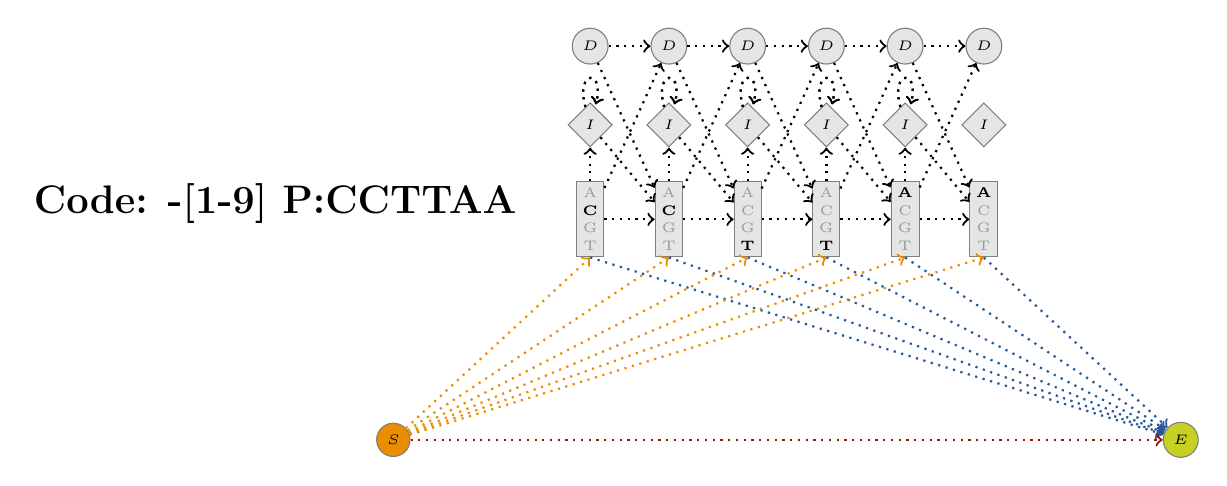
\begin{tikzpicture}
 \tiny
  \node  at (-2.5,1)  [font=\Large,style={align=center}] () {{\bf Code: -[1-9] P:CCTTAA}};
 
 \node[Dstate,fill=orange] (START) at (-1,-2){$S$};
\begin{scope}[shift={(1.5,2)}];

%CCTTAAGG
\node[Dstate] (dl1) at (0,1){$D$};
\node[Istate] (il1) at (0,0){$I$};
\node[Mstate] (ml1) at (0,-1.2){\shortstack{ {\color{black!40}A}\\  {\bf C} \\   {\color{black!40}G}\\ {\color{black!40}T}} };

\node[Dstate] (dl2) at (1,1){$D$};
\node[Istate] (il2) at (1,0){$I$};
\node[Mstate] (ml2) at (1,-1.2){\shortstack{ {\color{black!40}A}\\   {\bf C}\\   {\color{black!40}G}\\   {\color{black!40}T}} };

\node[Dstate] (dl3) at (2,1){$D$};
\node[Istate] (il3) at (2,-0){$I$};
\node[Mstate] (ml3) at (2,-1.2){\shortstack{ {\color{black!40}A}\\   {\color{black!40}C}\\   {\color{black!40}G}\\   {\bf T}} };

\node[Dstate] (dl4) at (3,1){$D$};
\node[Istate] (il4) at (3,0){$I$};
\node[Mstate] (ml4) at (3,-1.2){\shortstack{ {\color{black!40}A}\\   {\color{black!40}C}\\   {\color{black!40}G}\\   {\bf T}} };

\node[Dstate] (dl5) at (4,1){$D$};
\node[Istate] (il5) at (4,0){$I$};
\node[Mstate] (ml5) at (4,-1.2){\shortstack{ {\bf A}\\   {\color{black!40}C}\\   {\color{black!40}G}\\   {\color{black!40}T}} };

\node[Dstate] (dl6) at (5,1){$D$};
\node[Istate] (il6) at (5,-0){$I$};
\node[Mstate] (ml6) at (5,-1.2){\shortstack{ {\bf A}\\   {\color{black!40}C}\\   {\color{black!40}G}\\   {\color{black!40}T}} };
\end{scope}

\begin{scope}[shift={(9,-2)}];
\node[Dstate,fill=yellowgreen] (END) at (0,0){$E$};
\end{scope}


 \path

%(START)  edge [lightedge] (ml1)
(ml1) edge [lightedge] (ml2) 
(ml1) edge [lightedge] (dl2) 
(ml1) edge [lightedge] (il1)
   
(il1) edge [lightedge,loop above] ()
(il1) edge  [lightedge] (ml2)
(il1) edge [lightedge, loop above] ()
(dl1) edge  [lightedge,->] (dl2)
(dl1) edge  [lightedge,->] (ml2)

(ml2) edge [lightedge] (ml3) 
(ml2) edge [lightedge] (dl3) 
(ml2) edge [lightedge] (il2)
   
(il2) edge [lightedge,loop above] ()
(il2) edge  [lightedge] (ml3)
(il2) edge [lightedge, loop above] ()
(dl2) edge  [lightedge,->] (dl3)
(dl2) edge  [lightedge,->] (ml3)


(ml3) edge [lightedge] (ml4) 
(ml3) edge [lightedge] (dl4) 
(ml3) edge [lightedge] (il3)
   
(il3) edge [lightedge,loop above] ()
(il3) edge  [lightedge] (ml4)
(il3) edge [lightedge, loop above] ()
(dl3) edge  [lightedge,->] (dl4)
(dl3) edge  [lightedge,->] (ml4)


(ml4) edge [lightedge] (ml5) 
(ml4) edge [lightedge] (dl5) 
(ml4) edge [lightedge] (il4)
   
(il4) edge [lightedge,loop above] ()
(il4) edge  [lightedge] (ml5)
(il4) edge [lightedge, loop above] ()
(dl4) edge  [lightedge,->] (dl5)
(dl4) edge  [lightedge,->] (ml5)



(ml5) edge [lightedge] (ml6) 
(ml5) edge [lightedge] (dl6) 
(ml5) edge [lightedge] (il5)
   
(il5) edge [lightedge,loop above] ()
(il5) edge  [lightedge] (ml6)
(il5) edge [lightedge, loop above] ()
(dl5) edge  [lightedge,->] (dl6)
(dl5) edge  [lightedge,->] (ml6)


(ml1.south)edge [blue,lightedge] (END)
(ml2.south)edge [blue,lightedge] (END)
(ml3.south)edge [blue,lightedge] (END)
(ml4.south)edge [blue,lightedge] (END)
(ml5.south)edge [blue,lightedge] (END)
(ml6.south)edge [blue,lightedge] (END)

(START)edge [orange,lightedge] (ml1.south)
(START)edge [orange,lightedge] (ml2.south)
(START)edge [orange,lightedge] (ml3.south)
(START)edge [orange,lightedge] (ml4.south)
(START)edge [orange,lightedge] (ml5.south)
(START)edge [orange,lightedge] (ml6.south)
(START)edge [winered,lightedge] (END)

;

\end{tikzpicture}
\end{figure}




\chapter{Examples: putting it all together}

Here are some examples: 

\section{A library containing both barcodes and a 8 nucleotide fingerprint.}

In this example we expect the sequenced reads to contain a 6 nucleotide barcode sequence (out of a selection of 8) followed by a 8 nucleotide fingerprint, followed by the spacer sequence `TATA` followed by the read. \\

Here is the corresponding TagDust command: 


{\small
\begin{verbatim}
bash-3.1$ tagdust test.fq.gz   -1 O:N -2 :ACAGAT,ATCGTG,CACGAT,CACTGA,CTGACG,GAGTGA,GTATAC,TCGAGC
-3 F:NNNNNNNN -4 S:TATA -5 R:N  -o output.fq
\end{verbatim}
}

Note that we added an optional state at the beginning of the read in case extra nucleotides were added before the barcode.  \\ 

To remove ribosomal reads simply add the -ref and -fe options:

{\small
\begin{verbatim}
bash-3.1$ tagdust test.fq.gz   -1 O:N -2 :ACAGAT,ATCGTG,CACGAT,CACTGA,CTGACG,GAGTGA,GTATAC,TCGAGC
-3 F:NNNNNNNN -4 S:TATA -5 R:N  -o output.fq -ref U13369.1.fa -fe 2 
\end{verbatim}
}




\section{A RNA-seq library with a 'spaced' fingerprint.}

Here I downloaded a dataset from \cite{Kivioja:2012kg}. Reads start after the following construct:

{
\begin{verbatim}
T(NNN)dU(NNNN)dU(NNN)[GACTT]rGrGrGrG
\end{verbatim}
}
dU and rG represent deoxyuridine and guanine ribonucleotide, respectively. N's in brackets are the fingerprint nucleotides while GACTT is the barcode used. As you can see the ten nucleotide fingerprint is split into 3 parts separated by T's. \\

Here is the corresponding TagDust command: 


{\small
\begin{verbatim}

bash-3.1$ tagdust ERR048990.fastq  -1 F:NNN -2 S:T -3 F:NNNN -4 S:T -5 F:NNN -6 B:GACTT
-7 S:GGGG -8 R:N -start 1 -end 25  -o output.fq
\end{verbatim}
}

Note on the last line I restricted the search to the first 25 nucleotides for efficiency. 

\chapter{Algorithm}

\section{Sequence scoring} 

In short read mapping the mapping quality Q reflects the confidence we have in one particular mapping location over all others \cite{Li:2008ip}. Analogously, TagDust2 compares the probability of each read matching to the user specified HMM to the total summed probability including a random model:

\begin{equation}
P = 1 - \frac{P(x|M)*V}{P(x|M) + P(x|R)}
\end{equation} 

where $P(x|M)$ is the total summed probability of a read matching the model derived by the forward algorithm and $P(x|R)$ is the probability of the read give a random zero order Markov model. $V$ represents the fraction of $P(x|M)$ corresponding to the most likely barcode sequence. It is derived by using the backward and forward algorithm at each mutual exclusive transition:

\begin{equation}
	V = \max_j \left( \frac{f_s(i)   a_{s,m_j} e_{m_j}(x+1) b_{m_j}(i+1)}{\sum\limits_{\pi} P(x,\pi | M )}\right)
\end{equation}

where $ a_{s,m_j}$ is the transition from a silent to the first match state $m_j$ of a HMM modeling a barcode.  
 


\section{Implementation} 

Internally, TagDust uses a full profile HMM for each building block. We simply set some transition probabilities to zero to emulate different models. For example the read building block 'R' is implemented as a profile HMM with one column and transitions directly to and from the insertion state.
This is fairly inefficient as the dynamic programming code still needs to evaluate all possible transitions, even those we know in advance have a probability of zero. In future I might do something about this. 

\section{Optimal accuracy decoding} 

To obtain the most probably labeling of the sequence, we employ the optimal accuracy decoding algorithm as described in \citep{Kall:2005vg}. To apply this algorithm to our problem define the label probability of a nucleotide by the summed posterior label probabilities of states belonging to a particular HMM building block. A secondary dynamic programming algorithm is used to determine the path with the maximal label probability, constrained by the global HMM architecture. The label probabilities are essentially used as a substitution matrix while the architecture is enforced by the equivalent of gap penalties. 

If fingerprints are present TagDust checks at this stage if the length after decoding matches the users input. If not the read is discarded. 



%\chapter{Acknowledgements }


\begin{comment}
\chapter{hshsaer}
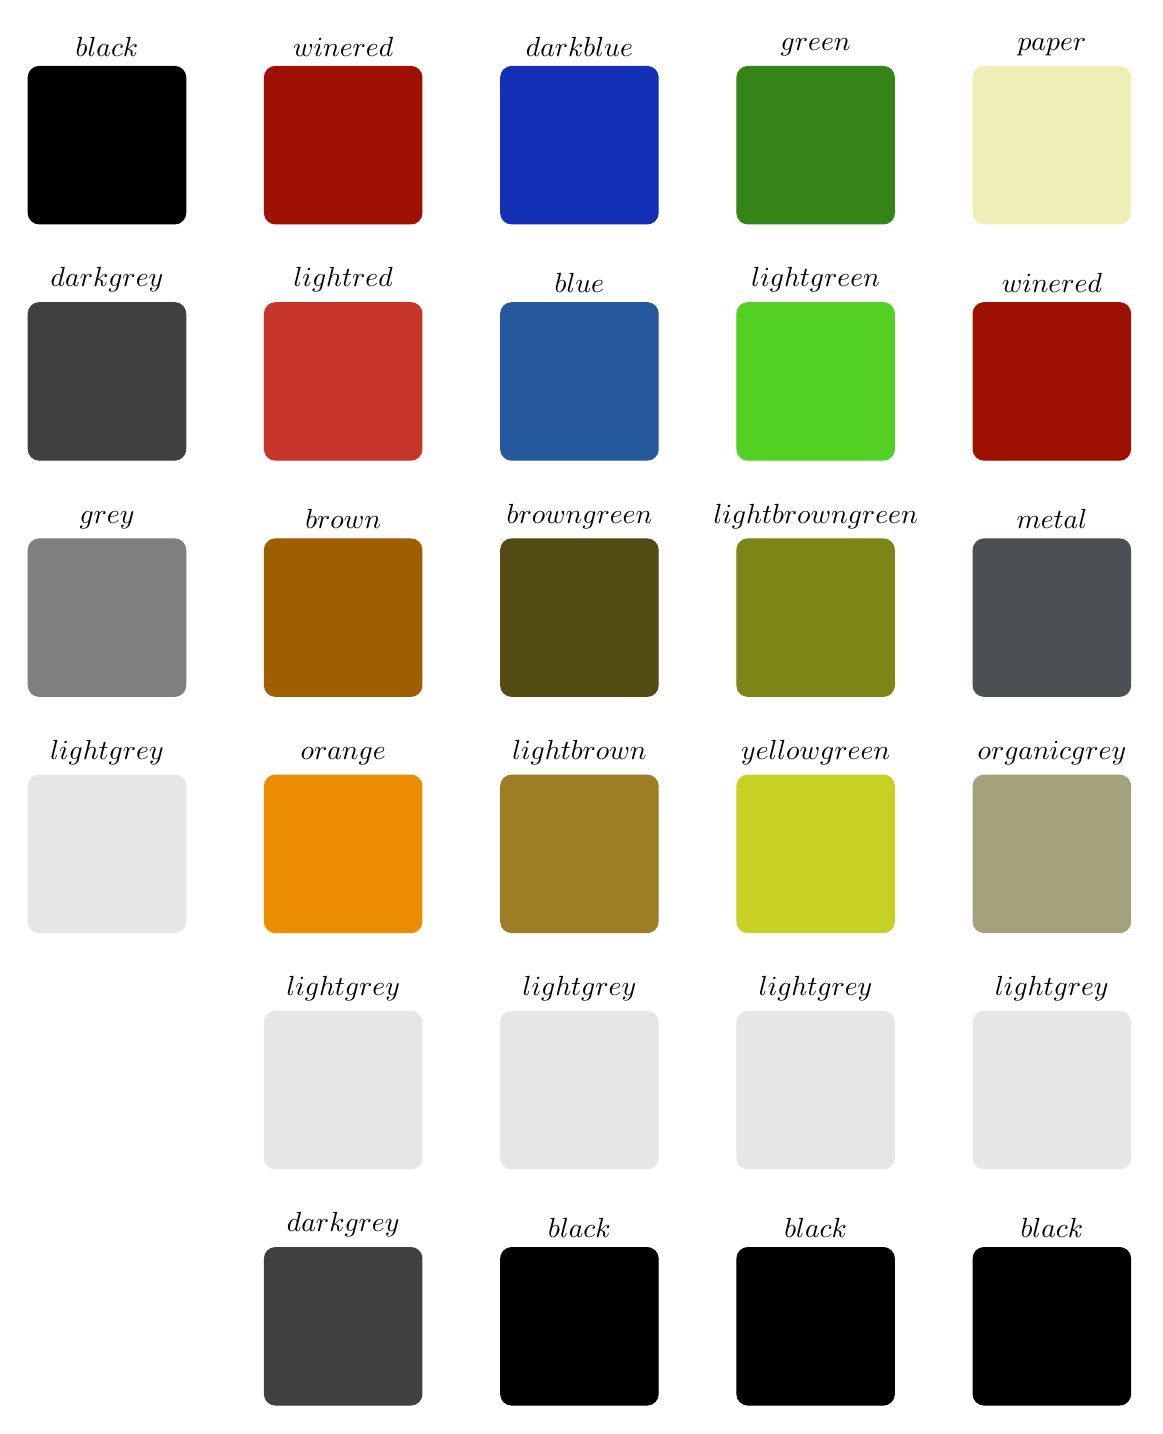
\begin{tikzpicture}[]
%\definecolor{black}{RGB}{0,0,0}
%\definecolor{darkgrey}{RGB}{64,64,64}
%\definecolor{grey}{RGB}{127,127,127}
%\definecolor{lightgrey}{RGB}{230,230,230}
\node [draw=black, fill=black,rounded corners=4pt,draw,rectangle,minimum width=2cm,minimum height=2cm,label=$black$] at (0,0) {};

\node [draw=darkgrey, fill=darkgrey,rounded corners=4pt,draw,rectangle,minimum width=2cm,minimum height=2cm,label=$darkgrey$] at (0,-3) {};

\node [draw=grey, fill=grey,rounded corners=4pt,draw,rectangle,minimum width=2cm,minimum height=2cm,label=$grey$] at (0,-6) {};

\node [draw=lightgrey, fill=lightgrey,rounded corners=4pt,draw,rectangle,minimum width=2cm,minimum height=2cm,label=$lightgrey$] at (0,-9) {};

%\definecolor{winered}{RGB}{158,16,0}
%\definecolor{ligthred}{RGB}{199,53,42}
%\definecolor{brown}{RGB}{158,95,0}
%\definecolor{orange}{RGB}{235,141,0}
\begin{scope}[shift={(3,0)}];
\node [draw=winered, fill=winered,rounded corners=4pt,draw,rectangle,minimum width=2cm,minimum height=2cm,label=$winered$] at (0,0) {};

\node [draw=lightred, fill=lightred,rounded corners=4pt,draw,rectangle,minimum width=2cm,minimum height=2cm,label=$lightred$] at (0,-3) {};

\node [draw=brown, fill=brown,rounded corners=4pt,draw,rectangle,minimum width=2cm,minimum height=2cm,label=$brown$] at (0,-6) {};

\node [draw=orange, fill=orange,rounded corners=4pt,draw,rectangle,minimum width=2cm,minimum height=2cm,label=$orange$] at (0,-9) {};

\node [draw=lightgrey, fill=lightgrey,rounded corners=4pt,draw,rectangle,minimum width=2cm,minimum height=2cm,label=$lightgrey$] at (0,-12) {};

\node [draw=darkgrey, fill=darkgrey,rounded corners=4pt,draw,rectangle,minimum width=2cm,minimum height=2cm,label=$darkgrey$] at (0,-15) {};

\end{scope}


%\definecolor{darkblue}{RGB}{19,48,182}

%\definecolor{blue}{RGB}{36,89,158}
%\definecolor{browngreen}{RGB}{82,75,19}
%\definecolor{lightbrown}{RGB}{158,126,36}

\begin{scope}[shift={(6,0)}];
\node [draw=darkblue, fill=darkblue,rounded corners=4pt,draw,rectangle,minimum width=2cm,minimum height=2cm,label=$darkblue$] at (0,0) {};

\node [draw=blue, fill=blue,rounded corners=4pt,draw,rectangle,minimum width=2cm,minimum height=2cm,label=$blue$] at (0,-3) {};

\node [draw=browngreen, fill=browngreen,rounded corners=4pt,draw,rectangle,minimum width=2cm,minimum height=2cm,label=$browngreen$] at (0,-6) {};

\node [draw=lightbrown, fill=lightbrown,rounded corners=4pt,draw,rectangle,minimum width=2cm,minimum height=2cm,label=$lightbrown$] at (0,-9) {};

\node [draw=lightgrey, fill=lightgrey,rounded corners=4pt,draw,rectangle,minimum width=2cm,minimum height=2cm,label=$lightgrey$] at (0,-12) {};

\node [draw=black, fill=black,rounded corners=4pt,draw,rectangle,minimum width=2cm,minimum height=2cm,label=$black$] at (0,-15) {};

\end{scope}

%\definecolor{green}{RGB}{52,132,23}
%\definecolor{lightgreen}{RGB}{82,209,36}
%\definecolor{lightbrowngreen}{RGB}{125,133,23}
%\definecolor{yellowgreen}{RGB}{198,209,36}


\begin{scope}[shift={(9,0)}];
\node [draw=green, fill=green,rounded corners=4pt,draw,rectangle,minimum width=2cm,minimum height=2cm,label=$green$] at (0,0) {};

\node [draw=lightgreen, fill=lightgreen,rounded corners=4pt,draw,rectangle,minimum width=2cm,minimum height=2cm,label=$lightgreen$] at (0,-3) {};

\node [draw=lightbrowngreen, fill=lightbrowngreen,rounded corners=4pt,draw,rectangle,minimum width=2cm,minimum height=2cm,label=$lightbrowngreen$] at (0,-6) {};

\node [draw=yellowgreen, fill=yellowgreen,rounded corners=4pt,draw,rectangle,minimum width=2cm,minimum height=2cm,label=$yellowgreen$] at (0,-9) {};

\node [draw=lightgrey, fill=lightgrey,rounded corners=4pt,draw,rectangle,minimum width=2cm,minimum height=2cm,label=$lightgrey$] at (0,-12) {};

\node [draw=black, fill=black,rounded corners=4pt,draw,rectangle,minimum width=2cm,minimum height=2cm,label=$black$] at (0,-15) {};

\end{scope}

%\definecolor{paper}{RGB}{240,238,183}
%\definecolor{organicgrey}{RGB}{163,162,124}
%\definecolor{metal}{RGB}{75,81,82}

\begin{scope}[shift={(12,0)}];
\node [draw=paper, fill=paper,rounded corners=4pt,draw,rectangle,minimum width=2cm,minimum height=2cm,label=$paper$] at (0,0) {};

\node [draw=winered, fill=winered,rounded corners=4pt,draw,rectangle,minimum width=2cm,minimum height=2cm,label=$winered$] at (0,-3) {};

\node [draw=metal, fill=metal,rounded corners=4pt,draw,rectangle,minimum width=2cm,minimum height=2cm,label=$metal$] at (0,-6) {};

\node [draw=organicgrey, fill=organicgrey,rounded corners=4pt,draw,rectangle,minimum width=2cm,minimum height=2cm,label=$organicgrey$] at (0,-9) {};

\node [draw=lightgrey, fill=lightgrey,rounded corners=4pt,draw,rectangle,minimum width=2cm,minimum height=2cm,label=$lightgrey$] at (0,-12) {};

\node [draw=black, fill=black,rounded corners=4pt,draw,rectangle,minimum width=2cm,minimum height=2cm,label=$black$] at (0,-15) {};


\end{scope}


%\draw[rounded corners=4pt,draw=hgrey, fill=hlightblue] (0,-6)	rectangle (+1,+1);
%\draw[rounded corners=4pt,draw=hgrey, fill=hlightblue] (0,-9)	rectangle (+1,+1);




\end{tikzpicture}
\end{comment}
\newpage
  
%-----------------------------------------------------------
\addcontentsline{toc}{chapter}{\numberline{}Bibliography}
\bibliographystyle{plain}
\bibliography{ref.bib}


%-----------------------------------------------------------
%\appendix
%
%\chapter{Long proofs}\label{app:proofs} An Appendix is a good place
%to put lengthy proofs that must be included but would impede the
%flow if placed in the main text.
%\section{Proof of theorem}\label{pf:angels}
%By inspection.

%-----------------------------------------------------------
\end{document}
